% ********** Приклад оформлення пояснювальної записки **********
% *********  до атестаційної роботи ступеня бакалавра **********
% ************* автори: Тавров Д. Ю., Сахаров С. Ю. ************

% зазначаємо стильовий файл, який будемо використовувати

\documentclass{bachelor_thesis}
% \usepackage{fontspec}


\usepackage{verbatim}
\usepackage{wrapfig}
\newcommand{\Mod}[1]{\ (\text{mod}\ #1)}
\renewcommand{\floatpagefraction}{.8}
\DeclareMathOperator{\ind}{ind}


\theoremstyle{definition}
\newtheorem{definition}{Визначення}[chapter]

% починаємо верстку документа
\begin{document}


% % !TEX root = ../abstract.tex
% створюємо анотацію
\setcounter{page}{4}
\chapter*{Реферат}
\pagestyle{plain}
\setfontsize{14}
% далі пишемо текст анотації

% анотація повинна починатися інформацією про структуру роботи
% (кількість аркушів (БЕЗ ДОДАТКІВ!), додатків, посилань, рисунків і таблиць)
Дипломну роботу виконано на 56 аркушах, вона містить 2 додатки та перелік посилань на використані джерела з 29 найменувань. У роботі наведено 6 рисунків та 3 таблиці.

% далі потрібно вказати мету роботи
Метою даної дипломної роботи є виконання алгоритмів дискретного логарифмування для мультиплікативних груп простих полів $GF(p)$ у хмарній моделі обчислень та оцінка дійсного розміру проблеми, яку можливо розв'язати з їх використанням за певний період часу та матеріальних витрат на цей розв'язок.

\textbf{Об'єктом дослідження} є проблема дискретного логарифму у скінченних полях виду $GF(p)$.

\textbf{Предметом дослідження} є процес виконання конкретних алгоритмів дискретного логарифмування у заданих полях на хмарних платформах.

% далі потрібно вказати розглянуті методи та критерії, за яким вибрано один із них
Проведено аналіз існуючих рішень проблеми дискретного логарифму, виконано їх порівняння з погляду швидкодії та легкості реалізації для паралельної моделі. Також проведено огляд існуючих систем хмарних обчислень та обрано ту, що дозволяє точніший контроль за загальною обчислювальною потужністю системи вузлів, з меншою ціною за рівних інших показниках. 

% далі потрібно коротко викласти суть роботи
Був реалізований обраний алгоритм у паралельній моделі та проведено його виконання на обраній платформі. З результатів виконання зроблено аналіз оптимальних параметрів алгоритму та орієнтовного розміру модуля, розв'язок проблеми дискретного логарифму для якого можна отримати за календарний рік.


Результати роботи можуть бути використані для оцінки вартості атаки на популярні асиметричні криптосистеми.

% наприкінці анотації потрібно зазначити ключові слова
\MakeUppercase{дискретний логарифм, index-calculus, паралельні обчислення, хмарні системи}

\chapter*{РЕФЕРАТ}
\pagestyle{plain}
Дипломная работа выполнена на 56 листах, она содержит 2 приложения и список ссылок на использованные источники с 29 наименований. В работе приведены 6 рисунков и 3 таблицы.

Целью данной дипломной работы является выполнение алгоритмов дискретного логарифмирования для мультипликативных групп простых полей $GF(p)$ в облачной модели вычислений и оценка действительного размера проблемы, которую можно решить с их использованием за определенный период времени и материальных затрат на это решение.

\textbf{Объектом исследования} является проблема дискретного логарифма в конечных полях вида $GF(p)$.

\textbf{Предметом исследования} является процесс выполнения конкретных алгоритмов дискретного логарифмирования в заданных полях на облачных платформах.

Проведен анализ существующих решений проблемы дискретного логарифма, выполнено их сравнение с точки зрения быстродействия и легкости реализации для параллельной модели. Также проведен осмотр существующих систем облачных вычислений и избран ту, что позволяет точнее контроль за общей вычислительной мощностью системы узлов, с меньшей ценой за равных других показателях.

Был реализован выбранный алгоритм в параллельной модели и проведено его выполнения на избранной платформе. С результатов выполнения сделано анализ оптимальных параметров алгоритма и ориентировочно размера модуля, решение проблемы дискретного логарифма для которого можно получить за календарный год.

Результаты работы могут быть использованы для оценки стоимости атаки на популярные асимметричные криптосистемы.

\MakeUppercase{Дискретный логарифм, INDEX-CALCULUS, параллельные вычисления, облачные системы}

% створюємо анотацію англійською мовою
\chapter*{Abstract}
\pagestyle{plain}
% анотація повинна починатися інформацією про структуру роботи
% (кількість аркушів (БЕЗ ДОДАТКІВ!), додатків, посилань, рисунків і таблиць)
The thesis is presented in 56 pages. It contains 2 appendixes and bibliography of 29 references. Six figures and 3 tables are given in the thesis. 

% далі потрібно вказати мету роботи

The goal of the thesis is to implement algorithms of discrete logarithm for multiplicative groups of fields of the form $GF(p)$ in the cloud computational model and to estimate the actual problem size which is possible to solve during some predefined period of time and to estimate the costs for such solution.

\textbf{The object} is discrete logarithm problem in the finite fields of the form $GF(p)$.

\textbf{The subject} is the process of some discrete logarithm algorithms execution on cloud platforms.

% далі потрібно вказати розглянуті методи та критерії, за яким вибрано один із них

In the thesis, existing solutions to the discrete logarithm problem are analyzed. They are compared in terms of performance and ease of use in parallel computational models. Also existing cloud systems are analyzed and the one is chosen based on more granular control over the whole computational power with other things equal.

% далі потрібно коротко викласти суть роботи
The selected algoritm is implemented in parallel computation model and is executed on the selected  platform. From the results of this execution analysis of optimal algorithm parameters and approximate problem size solvable in the span of one calendar year were made.

% далі потрібно подати відомості про апробацію роботи


The results could be used for estimating attack cost on popular asymmetric cryptosystems.

% наприкінці анотації потрібно зазначити ключові слова
\MakeUppercase{discrete logarithm, index-calculus, parallel computation, cloud systems}

% створюємо зміст
% 
\includepdf[pages={-}]{abstract.pdf}
\pagenumbering{gobble}
\tableofcontents
\cleardoublepage
\pagenumbering{arabic}
\setcounter{page}{3}

% створюємо перелік умовних позначень, скорочень і термінів
% \input{chapters/shortings}
% !TEX root = ../thesis.tex
% створюємо вступ
\intro
\pagestyle{plain}

Проблеми, з якими людство може зіштовхнутися у майбутньому, цікавлять людину давно, а особливо --- з початком НТР та швидкого прогресу 
соціальних, економічних та наукових аспектів життя. Письменники (особливо письменники-фантасти) часто користуються 
свободою творення для побудови різних варіантів розвитку людства. Як приклад можна навести цикл оповідань Айзека 
Азімова "Я, робот" \cite{asimov1950robot}, у якому автор намагається осягнути питання, які виникнуть із появою розумних 
машин. 

Якщо звернутись до більш наукових джерел, можна теж побачити великий пласт різного ступеню підкріпленості роздумів про 
типи та розв'язки проблем майбутнього. Міждсциплінарну галузь, що має на меті дослідження майбутнього, називають 
\emph{футурологією}. Словник Merriam-Webster \cite{MerriamWebster2009} надає визначення футурології як науки, що 
розглядає майбутні можливості на основі теперішніх трендів (\emph{переклад авт.}).

Україна теж не залишається осторонь цього процесу. Сам факт фізичного
 розташування нашої країни у просторово-часовому континуумі робить
 настання майбутнього, а разом із тим пов'язаних проблем, неминучим. Залишається лише питання
 конкретного вигляду цих проблем та способів їхнього розв'язання.

 У даній роботі зроблено спробу огляду та систематизації українських національних проблем майбутнього.

% !TEX root = ../thesis.tex
% створюємо розділ
\chapter{Огляд}
\label{chap:distributedcomputation}

Має сенс більш детально розглянути проблеми, з якими наша нація може з деякою
імовірністю зіштовхнутися у майбутньому.

\pagestyle{plain}

    \section{Загальний огляд та класифікація}\label{sec:general}
        Питання, які Україні доведеться вирішувати через деякий час, природньо поділяються на два класи:

        \begin{enumerate}
            \item Загальнолюдські проблеми
            \item Специфічно українські проблеми
        \end{enumerate}
        
        Спробуємо дати класифікації підтипів, що мають місце у цих класах. 

        Загальнолюдські проблеми можна поділити на:

        \begin{enumerate}
            \item Економічні:
            \begin{itemize}
                \item Зміна структури зайнятості
                \item Зростання нерівності у доходах
            \end{itemize}

            \item Екологічні:
            \begin{itemize}
                \item Зменшення біорізноманіття
                \item Зміна клімату
                \item Забруднення довкілля
            \end{itemize}

            \item Соціальні:
            \begin{itemize}
                \item Неоднорідна освітня модернізація
                \item Масштабна урбанізація
                \item Гендерна нерівність
                \item Зростання політичного популізму
            \end{itemize}
        \end{enumerate}

        Поділ специфічних проблем для України може бути таким:

        \begin{enumerate}
            \item Економічні:
            \begin{itemize}
                \item Ресурсозалежність
                \item Відсутність іноваційності
            \end{itemize}

            \item Екологічні:
            \begin{itemize}
                \item Забруднення, зокрема гідроресурсів
                \item Наслідки Чорнобилю та проблема зберігання ядерних відходів
                \item Вичерпання лісоресурсу
            \end{itemize}

            \item Соціальні:
            \begin{itemize}
                \item Старіння населення та еміграція
                \item Застаріла освіта
                \item Війна з Російською Федерацією
                \item Внутрішня нестабільність і надмірна централізованість
            \end{itemize}
        \end{enumerate}

        Наведену класифікацію можна наочно відобразити у вигляді mind map --- ієрархічного
        способу подання інформації \cite{hopper2015practicing}. Згенерована за
        допомогою програми SimpleMind Lite \cite{simplemind} така mind map наведена на рисунку \ref{fig:mindmap}.

        \begin{figure}[!htp]
            \centering
            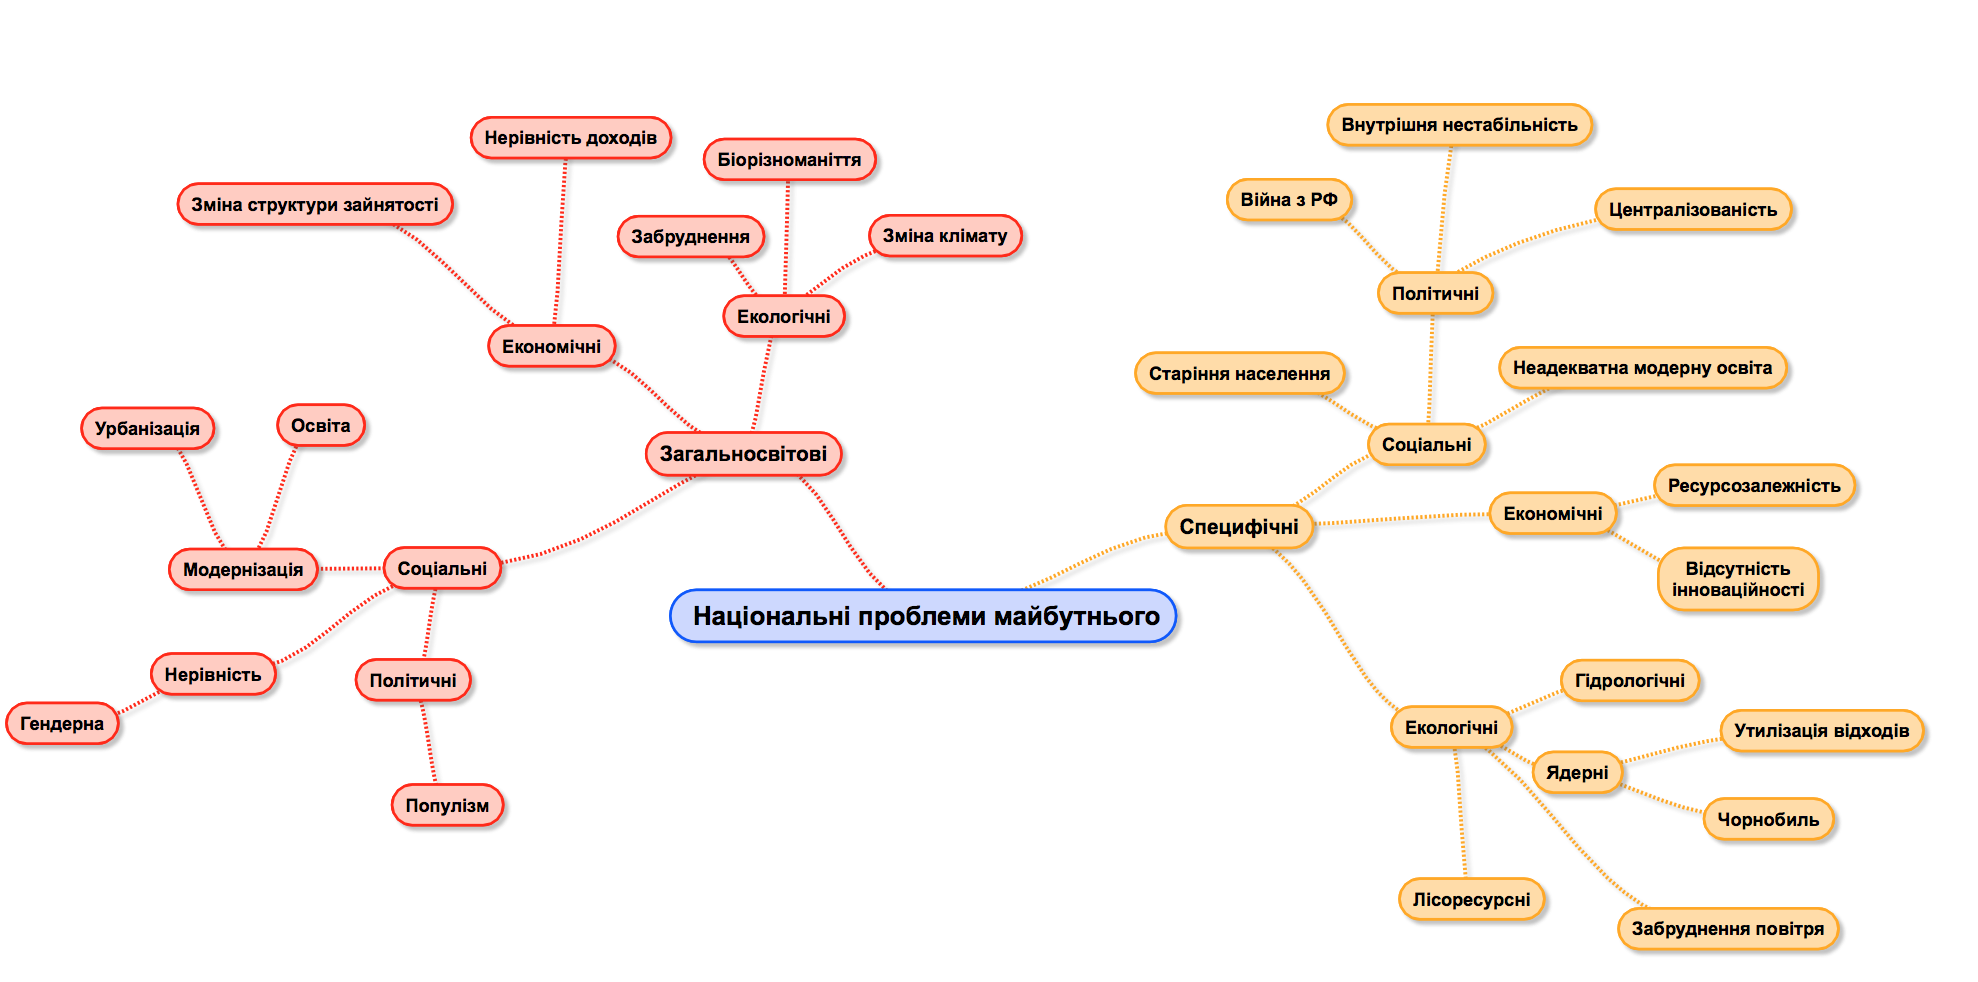
\includegraphics[scale = 0.5]{PNG/mindmap.png}
            \caption{Mind map}
            \label{fig:mindmap}
        \end{figure}


        Окреслимо деякі обрані проблеми більш детально у подальших підрозділах.

    \section{Загальнолюдські проблеми}\label{sec:world}


    \subsection{Зміна структури зайнятості}

        Завдяки прискоренню НТП (науково-технічного прогресу) все більше і більше процесів 
        у нашому житті стають автоматизованими. Машина здатна виконувати багато людських задач так само або краще,
        при цьому із констистентною продуктивністю та не потребуючи заробітньої платні(якщо, звісно, не вважати такою плату за
        спожиту електроенергію). Це, природньо, може призводити до повного або часткового зменшення кількості робочих місць для
        людей у окремих галузях.

        Журнал The Economist наводить інфографіку \cite{econinfo} кількості робочих місць у Сполучених Штатах Америки залежно від типу зайнятості
        з розбивкою по роках. Як типи зайнятості(типи виконуваної роботи) виділяються наступні:

        \begin{itemize}
            \item Рутинна розумова
            \item Рутинна фізична
            \item Нерутинна розумова
            \item Нерутинна фізична,
        \end{itemize}

        де під рутинною мається на увазі одноманітна тощо.

        % \begin{wrapfigure}{r}{0.5\textwidth}
        %     \begin{center}
        %       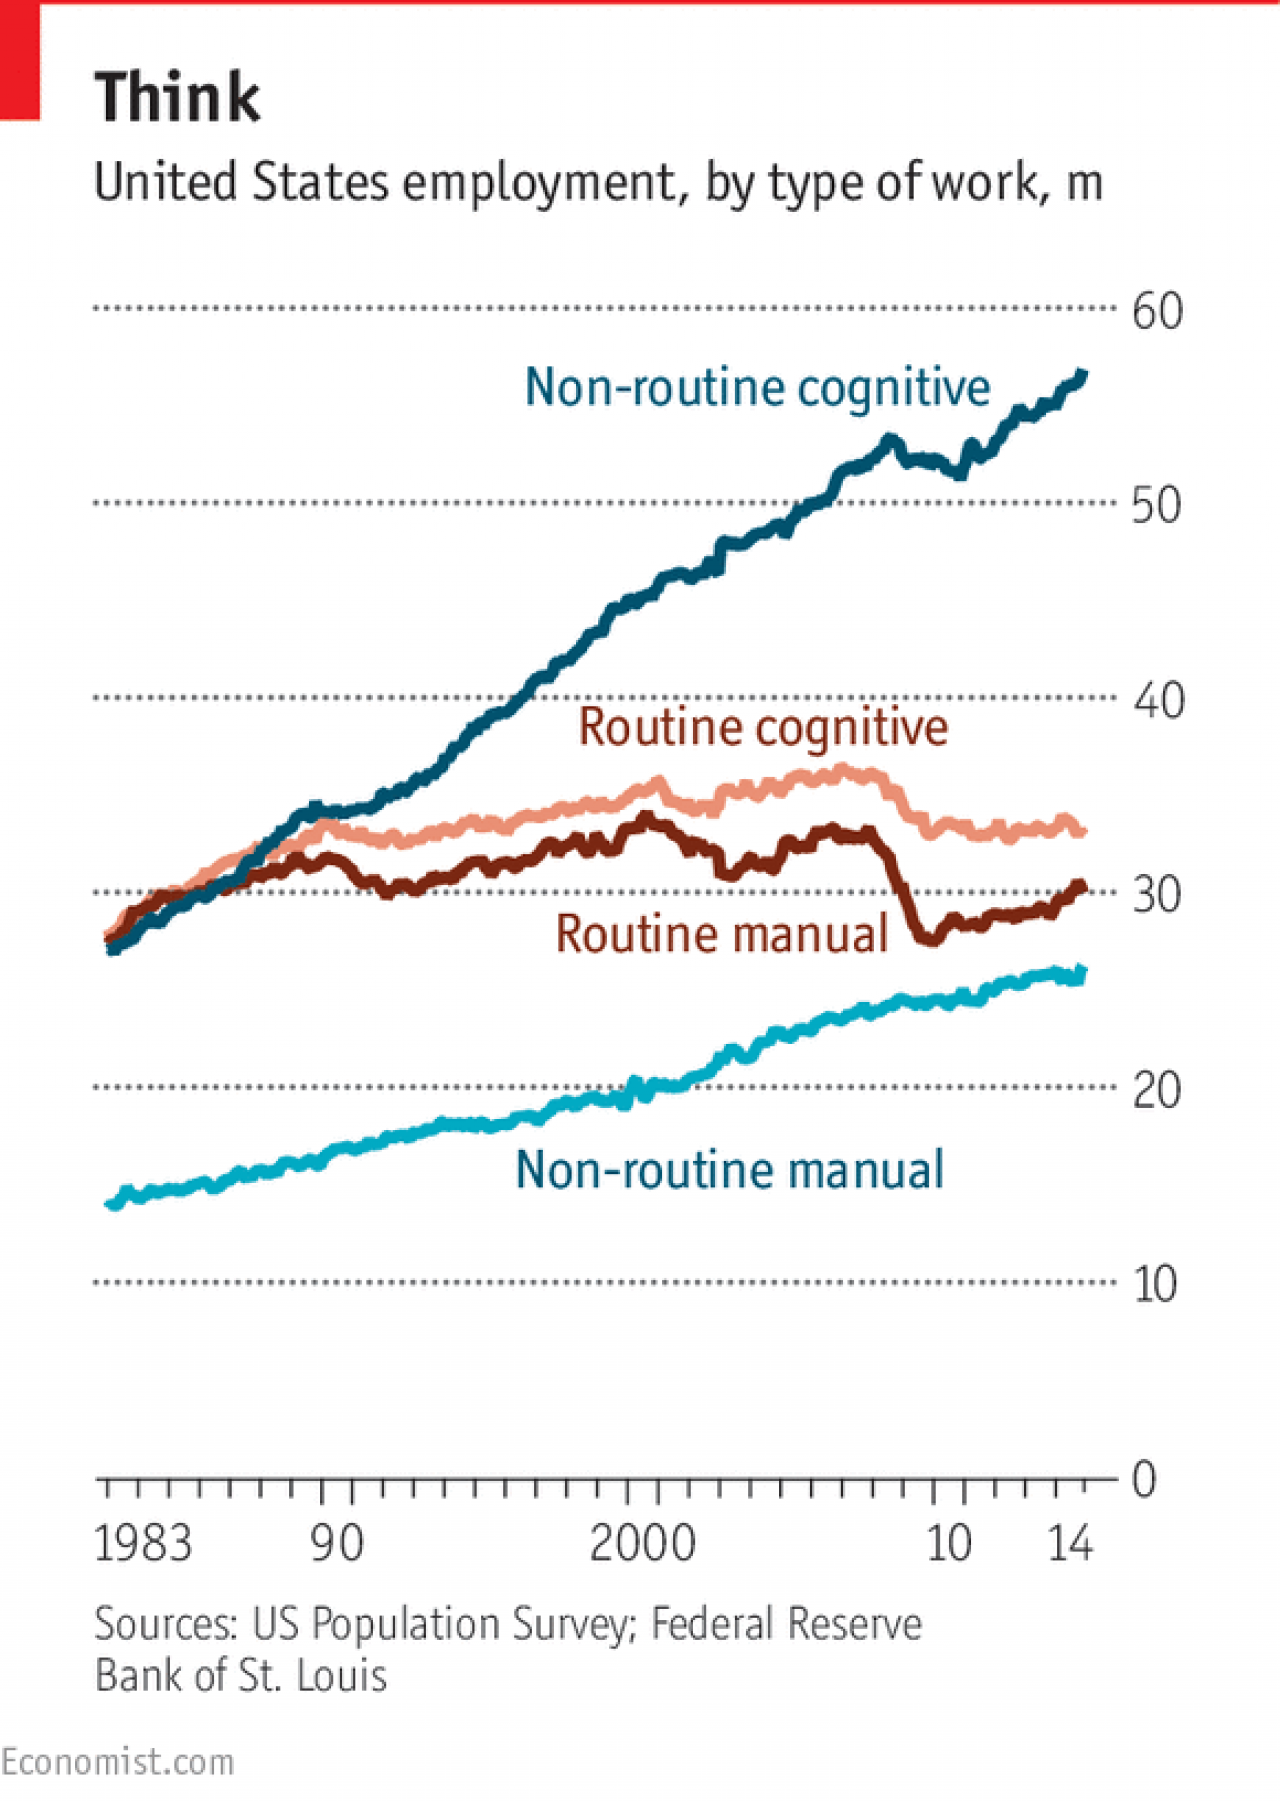
\includegraphics[width=0.48\textwidth]{PNG/economist.png}
        %     \end{center}
        %     \caption{Інфографіка The Economist}
        %     \label{fig:economist}            
        %   \end{wrapfigure}
          

        \begin{figure}[!htp]
            \centering
            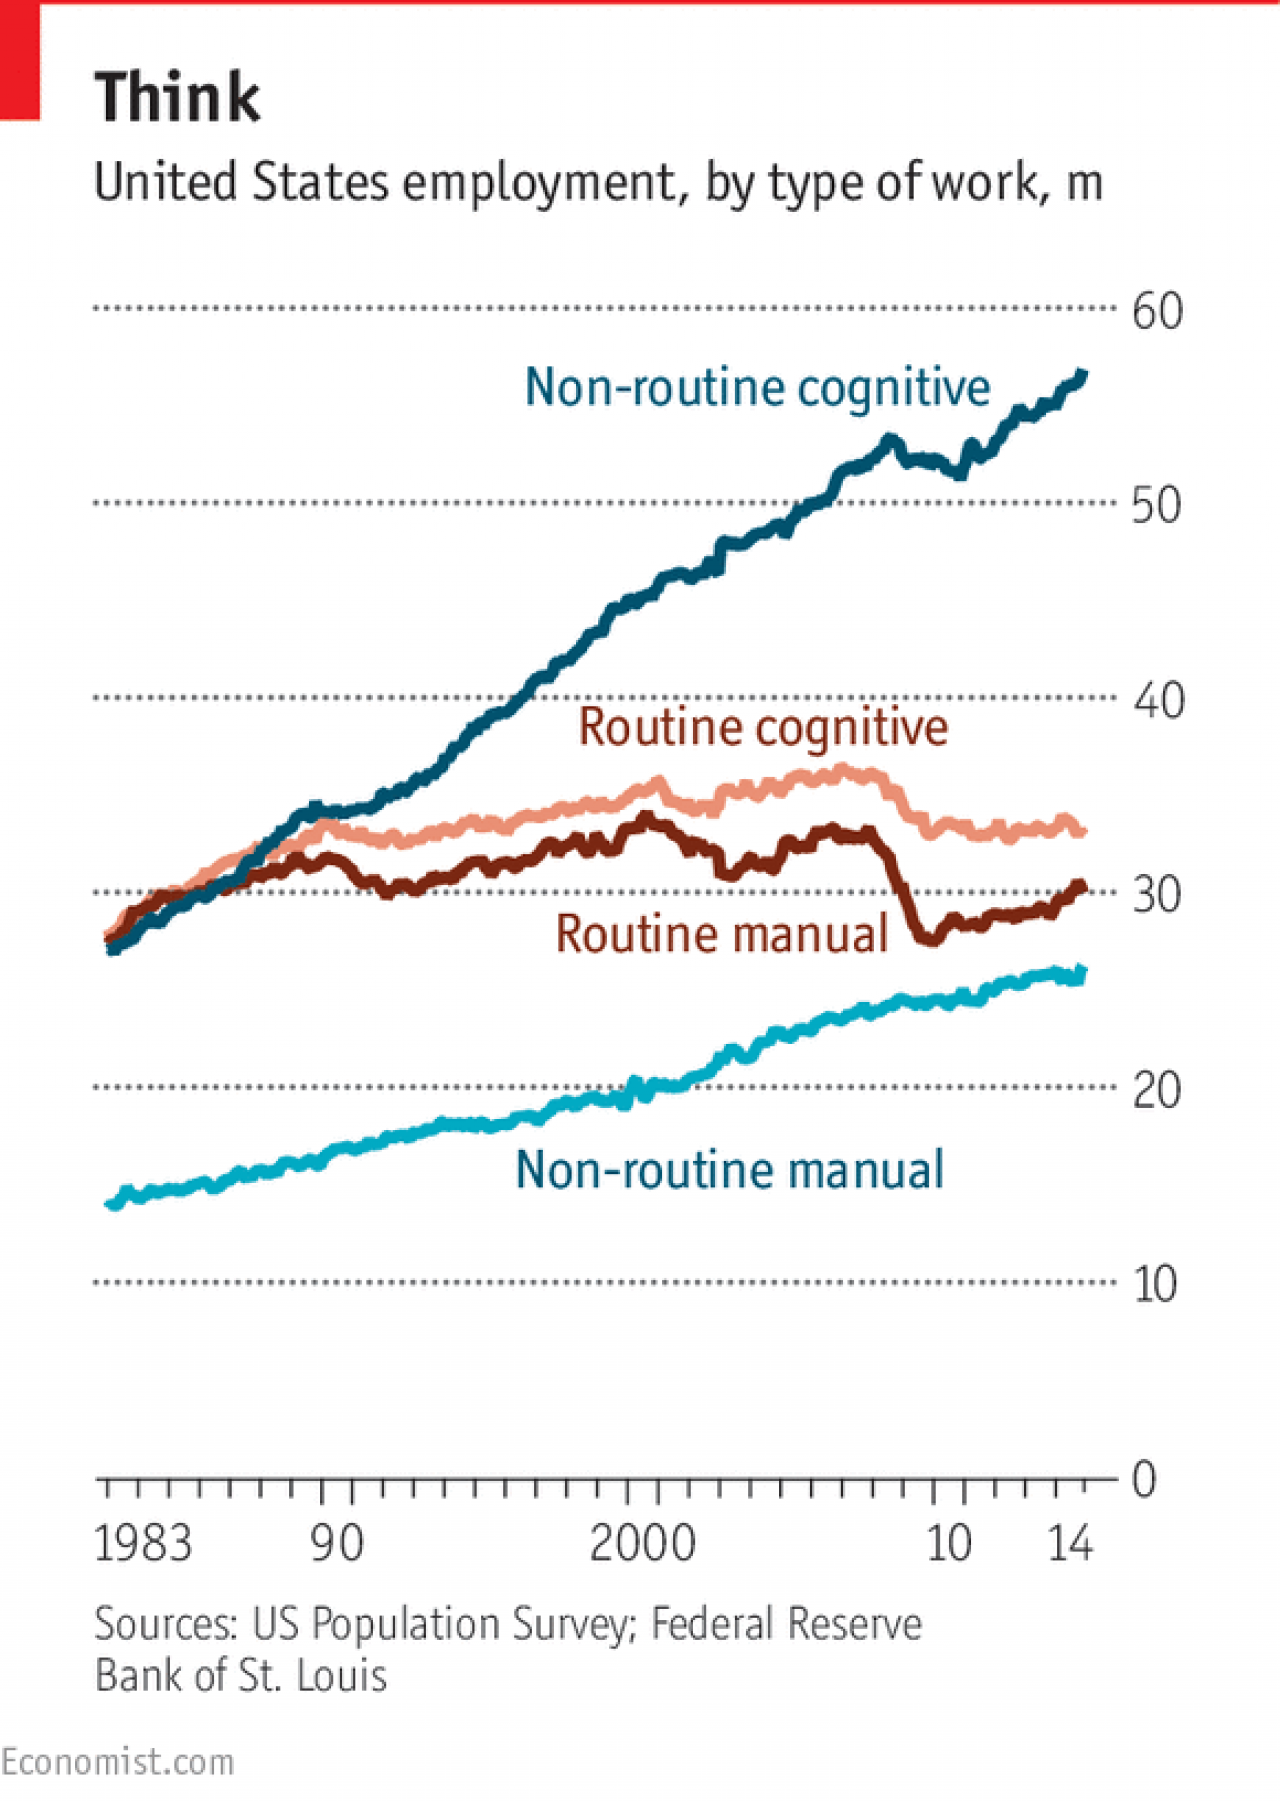
\includegraphics[scale = 0.19]{PNG/economist.png}
            \caption{Інфографіка The Economist}
            \label{fig:economist}
        \end{figure}

        З цієї інфографіки, яку можна побачити на рисунку \ref{fig:economist}, видно, що обсяги рутинних робочих місць перестають
        рости і навіть падають, у той час як обсяг нерутинних загалом не виявляє таких тенденцій. Доповідь PwC (PriceWater Coopers) 
        \cite{pwc} свідчить, що на початку 2030-х років 38 відсотків робочих місць у Сполучених Штатах будуть знаходитись під
        загрозою автоматизації.

        Враховуючи структуру зайнятості України \cite{ukrstatemployment}, для нашої країни ця проблема є ще більш нагальною. 
        Оскільки більшість населення працює фактично на рутинних роботах, можлива автоматизація має потенціал боляче вдарити по нашій
        економіці.

    \subsection{Зростання нерівності у доходах}
        
        Значною мірою зростанню соціальної напруженості сприяє нерівність у доходах населення. На рисунку \ref{fig:income_us}
        зображена астка доходів верхнього 1-го проценту людей у США по роках. Можна побачити наявність чіткого тренду на її зростання,
        тобто на зростання кількості ресурсів, якими володіє лише один відсоток населення (Зараз він становить майже 20\%)

        \begin{figure}[!htp]
            \centering
            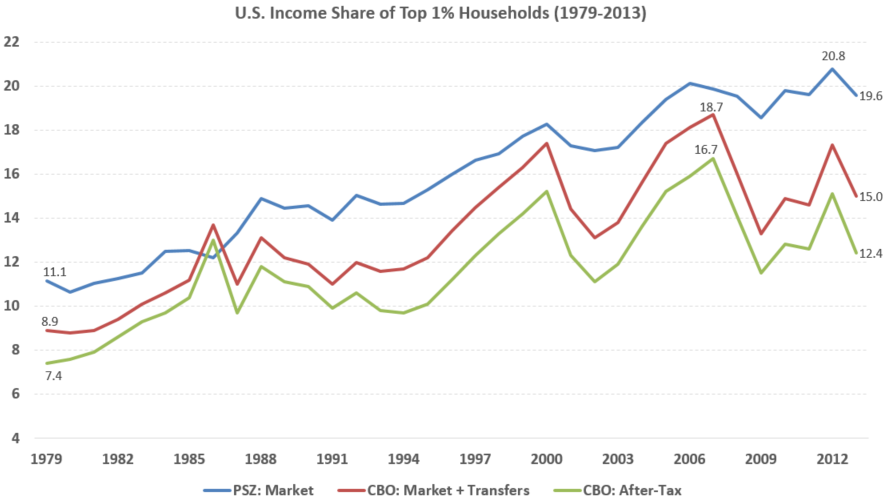
\includegraphics[scale = 0.7]{PNG/income_us.png}
            \caption{Частка доходів верхнього 1-го проценту людей у США по роках}
            \label{fig:income_us}
        \end{figure}

        Хоча нерівність в Україні поки що не показує динаміку до зростання (індекс Джині лишається стабільним, і навіть зменшується
        \cite{giniukr}), ця тенденція може не обминути стороною і нашу країну у майбутньому.

    \subsection{Змiна клiмату}

        У період з х до х року середня температура на Землі збільшилась на х (ц). Ця аномальна як на звичну поведінка 
        приголомшливою більшістю вчених (ц) пояснюється зміною клімату внаслідок людської діяльності. Обсяги СО2 у атмосфері зростають
        у першу чергу завдяки порушенню балансу через використання викопних джерел енергії. 

        (к)

        Незважаючи на думку наукової спільноти, велика кількість політиків відмовляється визнавати зміну клімату і навіть будє на цьому
        кар'єру. Президент чи не найбільшого забрудника - США - Дональд Трамп декілька разів публічно відмовлявся вірити у таку зміну (ц).
        Оскільки ця проблема не має меж і кордонів, для України вона теж є винятково важливо в тому числі і через те, що на наш добробут
        можуть напряму повпливати інші країни.

    \subsection{Зростання політичного популізму}

        Згадавши про Дональда Трампа, можна згадати і про одну з проблем, які він уособлює "--- зростання політичного популізму 
        по всьому світу
% \input{chapters/index_calculus}
% \input{chapters/real}

% висновки
%!TEX root = ../thesis.tex
% створюємо Висновки до всієї роботи
\conclusions

% \input{chapters/bibliography}
\bibliography{thesis}
\bibliographystyle{gost780s} 
% % створюємо додатки
% % перший додаток повинен містити лістинги розроблених програм
% \append{Лістинги програм}

% % кожний лістинг вставляється в додаток за допомогою спеціальної команди,
% % перший аргумент якої --- це заголовок, який з'являтиметься в тексті,
% % другий --- шлях до файлу з лістингом
% \listing{presenter.h --- прототип пред'явника-вчителя}{SRC/Presenter/presenter.h}

% \listing{presenter.cpp --- реалізація пред'явника-вчителя}{SRC/Presenter/presenter.cpp}

% \input{chapters/appendix_firstrun}

% % останній додаток повинен містити слайди презентації доповіді на захисті дипломної роботи
% \append{Ілюстративний матеріал}

% \begin{figure}[!htp]%
% 	\centering
% 	\includegraphics[scale = 0.43]{PNG/slide1.png}%
% 	\caption{Слайд 1}%
% 	\label{fig:p1}%
% \end{figure}

% \begin{figure}[!htp]%
% 	\centering
% 	\includegraphics[scale = 0.455]{PNG/slide2.png}%
% 	\caption{Слайд 2}%
% 	\label{fig:p2}%
% \end{figure}

\end{document}
